\documentclass[twoside]{article}
\usepackage{verbatim}
\usepackage{multirow} \usepackage{enumerate}
\usepackage{amsmath,enumerate} \usepackage{amsthm}
\usepackage{algcompatible}
\usepackage{algpseudocode}
\usepackage{algorithm}
%\usepackage{algorithmic}
%\usepackage{pstricks}
\usepackage{amssymb, latexsym}
\usepackage{xfrac}
\usepackage{mathtools}
\usepackage{graphicx}
\usepackage[captionskip=5pt, nearskip=5pt, font=small]{subfig}
\DeclareGraphicsRule{*}{mps}{*}{}
\usepackage{listings}

%specific to this document only
%\usepackage{pgfplots}
\usepackage{pgfplotstable}
\pgfplotstableread{plts/experiment_erdren_edgecolor.tab}\erdrenone
\pgfplotstableread{plts/experiment_erdren_edgecolor_400.tab}\erdrentwo
\pgfplotstableread{plts/experiment_erdren_directededgecolor.tab}\erddirone
\pgfplotstableread{plts/experiment_erdren_directededgecolor_400.tab}\erddirtwo
\pgfplotstableread{plts/experiment_sclfre_edgecolor.tab}\sclfreeone
\pgfplotstableread{plts/experiment_sclfre_edgecolor_400.tab}\sclfreetwo
\pgfplotstableread{plts/experiment_smlwld_edgecolor.tab}\smlwldone
\pgfplotstableread{plts/experiment_smlwld_edgecolor_64.tab}\smlwldtwo
\pgfplotstableread{plts/experiment_smlwld_edgecolor_256.tab}\smlwldthree
%\pgfplotstableread{plts/experiment8b2_av.tab}\averagetwo
%\pgfplotstableread{plts/experiment8b3_av.tab}\averagethree
%\pgfplotstableread{plts/experiment8b4_av.tab}\averagefour
%\pgfplotstableread{plts/experiment9a_av.tab}\stepping
%\pgfplotstableread{plts/experiment9a1_av.tab}\steppingone
%\pgfplotstableread{plts/experiment9a2_av.tab}\steppingtwo
%\pgfplotstableread{plts/experiment9a3_av.tab}\steppingthree
%\pgfplotstableread{plts/experiment9a4_av.tab}\steppingfour
%\pgfplotstableread{plts/experiment9b1_av.tab}\runningone
%\pgfplotstableread{plts/experiment9b2_av.tab}\runningtwo
%\pgfplotstableread{plts/experiment9b3_av.tab}\runningthree
%\pgfplotstableread{plts/experiment9b4_av.tab}\runningfour
%\pgfplotstableread{plts/experiment9b_av.tab}\running
%\pgfplotstableread{plts/experiment9c_av.tab}\costcomp
%\pgfplotstableread{plts/experiment9c1_av.tab}\costcompone
%\pgfplotstableread{plts/experiment9c2_av.tab}\costcomptwo
%\pgfplotstableread{plts/experiment9c3_av.tab}\costcompthree
%\pgfplotstableread{plts/experiment8b1_rn.tab}\runsone
%\pgfplotstableread{plts/experiment8b2_rn.tab}\runstwo
%\pgfplotstableread{plts/experiment8b3_rn.tab}\runsthree
%\pgfplotstableread{plts/experiment8b4_rn.tab}\runsfour
%\pgfplotstableset{
%  create on use/density/.style={
%    create col/expr={\thisrow{nodes}+\thisrow{links}}}
%    }
\pgfplotstableset{
  create on use/delta/.style={
    create col/expr={\thisrow{links}/\thisrow{nodes}}
    }}
%\pgfplotstableset{
%  create on use/nodebylinks/.style={
%    create col/expr={(\thisrow{nodes}*\thisrow{links})}}
%    }
%\pgfplotscreateplotcyclelist{three}{% 
%  every mark/.append style={fill=teal}\\% 
%  every mark/.append style={fill=green}\\% 
%  every mark/.append style={fill=orange}\\% 
%}
%\pgfplotscreateplotcyclelist{four}{%
%  every mark/.append style={fill=teal}\\%
%  every mark/.append style={fill=green}\\%
%  every mark/.append style={fill=orange}\\%
%  every mark/.append style={fill=pink}\\%
%}
%\pgfplotscreateplotcyclelist{three-1-0}{%
%  every mark/.append style={fill=teal}\\% 
%  every mark/.append style={fill=green}\\% 
%  every mark/.append style={fill=orange}\\%
%	every mark/.append style={fill=none}\\% 
%	every mark/.append style={fill=none}\\% 
%	every mark/.append style={fill=none}\\% 
%}
%\pgfplotscreateplotcyclelist{three-0-1}{%
%	every mark/.append style={fill=none}\\% 
%	every mark/.append style={fill=none}\\% 
%	every mark/.append style={fill=none}\\% 
%  every mark/.append style={fill=teal}\\% 
%  every mark/.append style={fill=green}\\% 
%  every mark/.append style={fill=orange}\\%
%}
%\pgfplotscreateplotcyclelist{four-1-0}{%
%  every mark/.append style={fill=teal}\\%
%  every mark/.append style={fill=green}\\%
%  every mark/.append style={fill=orange}\\%
%  every mark/.append style={fill=pink}\\%
%	every mark/.append style={fill=none}\\%
%	every mark/.append style={fill=none}\\%
%	every mark/.append style={fill=none}\\%
%	every mark/.append style={fill=none}\\%
%}
%\pgfplotscreateplotcyclelist{four-0-1}{%
%	every mark/.append style={fill=none}\\%
%	every mark/.append style={fill=none}\\%
%	every mark/.append style={fill=none}\\%
%	every mark/.append style={fill=none}\\%
%  every mark/.append style={fill=teal}\\%
%  every mark/.append style={fill=green}\\%
%  every mark/.append style={fill=orange}\\%
%  every mark/.append style={fill=pink}\\%
%}

%%%%%%%%%%%%%

\usepackage{pgf}
\usepackage{tikz}
\usetikzlibrary{decorations.pathmorphing} % LATEX and plain TEX when using Tik Z
\usetikzlibrary{positioning}
\usetikzlibrary{er}
\usetikzlibrary{automata}
\usetikzlibrary{shapes.geometric}
\usetikzlibrary{shapes.misc}
\tikzstyle{vx}=[draw,circle,fill=white,minimum size=2pt, inner sep=1pt, node distance=15mm]
\tikzstyle{ex}=[draw,rectangle,fill=white,minimum size=2pt, inner sep=3pt, node distance=15mm]
\tikzstyle{nfo}=[anchor=north west, rectangle, fill=white,text width=4cm, inner sep=3pt, node distance=15mm]
\tikzstyle{bup}=[semithick, decoration={bent, aspect=.3, amplitude=4}, decorate, ->, >=stealth]
\tikzstyle{bdn}=[semithick, decoration={bent, aspect=.3, amplitude=-4}, decorate, ->, >=stealth]
\tikzstyle{BUP}=[thick, decoration={bent, aspect=.3, amplitude=8}, decorate, ->, >=stealth]
\tikzstyle{BDN}=[thick, decoration={bent, aspect=.3, amplitude=-8}, decorate, ->, >=stealth]
\tikzstyle{MUP}=[thick, decoration={bent, aspect=.3, amplitude=16}, decorate, ->, >=stealth]
\tikzstyle{MDN}=[thick, decoration={bent, aspect=.3, amplitude=-16}, decorate, ->, >=stealth]
\tikzstyle{pln}=[draw, dotted]
\tikzstyle{dir}=[draw, dotted, decorate, ->, >=stealth, bend left=10]
\tikzstyle{str}=[semithick, decorate, ->, >=stealth]
\tikzstyle{cr}=[draw, circle, fill=black!25,minimum size=150pt]
\tikzstyle{rst}=[state, shape=rounded rectangle, rounded rectangle arc length=90, text width=2cm, inner sep=4pt]
\tikzstyle{rsf}=[state, fill=green!35, shape=rounded rectangle, rounded rectangle arc length=90, text width=1.75cm, inner sep=4pt]
%styles for plots?
\tikzstyle{bls}=[blue, solid, mark=square*]
\tikzstyle{grt}=[red, solid, mark=*]
\tikzstyle{inv}=[draw=none]

% \paperheight=11in \paperwidth=8.5in \textheight=9.0in
% \textwidth=6.5in \voffset=-.875in \hoffset=-.875in
\newenvironment{code} {\begin {quote}\begin{footnotesize}}
    {\end{footnotesize}\end{quote}}

% \oddsidemargin 0.0 in \evensidemargin 0.0 in
\newenvironment{enumeratealpha}
{\begin{enumerate}[(a{\textup{)}}]}{\end{enumerate}}

\theoremstyle{plain}
\newtheorem{lem-rule}{Rule}
\newtheorem{thm}{Theorem}
\newtheorem{con}{Conjecture}
\newtheorem{lem}{Lemma}[thm]
\newtheorem{prp}{Proposition}
\newtheorem{prop}{Proposition}[con]
\newtheorem{lprp}{Proposition}[lem]
\newtheorem{cor}{Corollary}[lem]
\theoremstyle{definition}
\newtheorem{defn}{Definition}[thm]
\newtheorem{defi}{Definition}
\newtheorem{dfn}{Definitions}[thm]
\newtheorem{ldef}{Definition}[lem]
\newtheorem{assm}{Assumption}
\theoremstyle{remark}
\newtheorem*{smy}{Summary}
\newtheorem{note}{Note}[thm]
\newtheorem{case}{Case}
%algorithms commands
\algblockdefx[Case]{Case}{EndCase} %
[1] [{\em var}] {{\bfseries case} {\em #1\ } } %
{{\bfseries end case}}%
\algcblockdefx[Case]{Case}{When}{EndCase}
[1] [{\em true}] {{\bfseries when} {\em #1\ }}
{{\bfseries end case}} %

\algblockdefx[TimesDo] {DoTimes}{EndTimes}
[1] [0] {#1 times {\bfseries do}}
{{\bfseries end do}}

%subalgorithms environment
\makeatletter
\newcounter{parentalgorithm}
\newenvironment{subalgorithms}{%
%  \refstepcounter{algorithm}%
  \floatname{algorithm}{Procedure}
  \protected@edef\theparentalgorithm{\thealgorithm}%
  \setcounter{parentalgorithm}{\value{algorithm}}%
  \setcounter{algorithm}{0}%
  \def\thealgorithm{\theparentalgorithm-\alph{algorithm}}%
  \ignorespaces
}{%
  \setcounter{algorithm}{\value{parentalgorithm}}%
  \ignorespacesafterend
}
\makeatother

%code environments
\usepackage{float}
 
\floatstyle{ruled}
\newfloat{codeblock}{thp}{lop}
\floatname{codeblock}{Example}

\lstnewenvironment{rubyblock} 
{\lstset{language=Ruby, breaklines=true, basicstyle=\small, xleftmargin=10pt, numbers=left, numberstyle=\tiny, stepnumber=1, numbersep=5pt, escapeinside={|;}{;|}}}
{}
% text macros
\def\cI{{\mathcal I}} \def\cR{{\mathcal R}} \def\cE{{\mathcal E}}
\def\cC{{\mathcal C}} \def\cF{{\mathcal F}} \def\cU{{\mathcal U}}
\def\cH{{\mathcal H}} \def\cD{{\mathcal D}} \def\cB{{\mathcal B}}
\def\cQ{{\mathcal Q}} \def\cV{{\mathcal V}} \def\cS{{\mathcal S}}
\def\cG{{\mathcal G}} \def\cA{{\mathcal A}} \def\cO{{\mathcal O}}
\def\cW{{\mathcal W}} \def\cL{{\mathcal L}} 

\def\bI{{\mathbb I}} \def\bO{{\mathbb O}}
\def\bC{{\mathbb C}} \def\bM{{\mathbb M}}
\def\bId{{$\mathbb I$}} \def\bOd{{$\mathbb O$}}
\def\bCd{{$\mathbb C$}} \def\bMd{{$\mathbb M$}}

\def\cId{{$\mathcal I$}} \def\cRd{{$\mathcal R$}} \def\cEd{{$\mathcal E$}} 
\def\cCd{{$\mathcal C$}} \def\cFd{{$\mathcal F$}} \def\cUd{{$\mathcal U$}} 
\def\cHd{{$\mathcal H$}} \def\cDd{{$\mathcal D$}} \def\cBd{{$\mathcal B$}} 
\def\cQd{{$\mathcal Q$}} \def\cVd{{$\mathcal V$}} \def\cSd{{$\mathcal S$}} 
\def\cGd{{$\mathcal G$}} \def\cAd{{$\mathcal A$}} \def\cOd{{$\mathcal O$}}
\def\cWd{{$\mathcal W$}} \def\cLd{{$\mathcal L$}}

\def\suchthat{{\: |\:}}




\usepackage{IJNC}


\setcounter{page}{501}
\newcommand{\jvolume}{X}
\newcommand{\jnumber}{Y}
\newcommand{\jmonth}{January}
\newcommand{\jyear}{20XX}

% title
\newcommand{\jtitle}{A General Purpose Automata for Distributed Graph Algorithms}
% running title for header
\newcommand{\jrunningtitle}{A General Purpose Automata}



\pagestyle{plain}


\begin{document}
\thispagestyle{empty}
\copyrightheader

\begin{center}
% print title
\jtitle

\vspace{20pt}

J. Paul Daigle 

\vspace{2pt}

Department of Computer Science, Georgia State University\\
Atlanta, GA, 30303, USA

\vspace{10pt}
%and
%
\vspace{10pt}
Sushil K. Prasad

\vspace{2pt}
Department of Computer Science, Georgia State University\\
Atlanta, GA, 30303, USA

\vspace{10pt}
%and
%
%\vspace{10pt}
%THIRD AUTHOR
%
%\vspace{2pt}
%Group, Laboratory, Address\\
%City, State ZIP, Country

\vspace{20pt}
\publisher{(received date)}{(revised date)}{(accepted date)}{Editor's name}
%\publisherA{(received date)}{(revised date)}{(revised date)}{(accepted date)}{Editor's name}

\end{center}


\begin{abstract}
We present an automata for a compute node in a message passing model which allows a distributed computer to approximate solutions for three NP-Complete graph problems. Our algorithm for the Vertex Cover Problem uses $O(\log{\Delta)}$ communication rounds to find a 2-approximate solution. Our edge coloring algorithm is also 2-approximate and resolves in $O(\Delta)$ rounds, and we find a correct strong edge coloring of a symmetric digraph in $O(\Delta)$ rounds. All three algorithms require only one hop information to find correct solutions. 
\keywords{Distributed Algorithms, Vertex Cover, Edge Coloring, Strong Edge Coloring}
\end{abstract}


\section{Introduction}

In this paper we expand on our prior work in \cite{Daigle:2011uq, Daigle:2012uq} using a simple Matching Automata to find constant approximations for NP-complete problems on a message passing computer. We present both theoretical and experimental results. We improve on our prior work in two ways, first, we improve our proof for correctness and performance, second, we present expanded experimental results, and third, we present an improved algorithm for edge color.


\subsection{Definitions}

\begin{defi}[Minimum Vertex Cover]
\label{sub:mvc}

Given an undirected Graph $G(V,E)$, a {\em Vertex Cover} of $G$ is a set of vertices $V'$ such that for each edge $e_{u,v} \in E$, $u \in V'$ or $v \in V'$. The Minimum Vertex Cover Problem is to find the smallest possible vertex cover of $G$.

\end{defi}

\begin{defi}[Minimum Weighted Vertex Cover]
\label{sub:mwvc}
Given an undirected Graph $G(V,E)$, where each $v \in V$ has a positive weight $w(v)$, minimize $\sum_{v \in V'} w(v)$.
\end{defi}

\begin{defi}[Edge Coloring]
\label{def:ec}
An edge coloring of a graph is an assignment of colors to the edges of a graph in such a way that no two adjacent edges are assigned the same color. 

Formally, given a graph, $G(V,E)$, and set of colors $C$, an edge coloring of $G$ is a mapping $f(e) = E \mapsto C \suchthat \forall\, e(u,v), e'(v,w) \in E, c \in C, f(e) = c \implies f(e') \ne c$.

\end{defi}


\begin{defi}[Strong Directed Edge Coloring]

A strong edge coloring is an assignment of colors to the edges of the graph such that no two edges that can be connected by a common edge are assigned the same color. 

In the directed case, a strong edge coloring is a mapping:
  \begin{align*} 
    f(e) = C \mapsto E \suchthat \forall\, e(u,v), e'(v,u), e''(w,v), e'''(w,x) \in E, c \in C,\\ 
    f(e) = c \implies f(e') \ne c, f(e'') \ne c, f(e''') \ne c 
  \end{align*} 
\end{defi}


\subsection{The Model and Automata}

\subsubsection{The Message Passing Model}
Our algorithms assume a message passing model of distributed computing. Therefore, we make the following two assumptions. First, communication rounds proceed synchronously. Second, each node can communicate with each of its neighbors once during any communication round. Structurally, our algorithms map each vertex of the graph to a compute node of the distributed computer. 

We also use the term `round' in two different senses. A computation round in our algorithm is composed of several communication rounds. Referring to the automata in Figure~\ref{fig:automata}, the automata defines the possible states of a node during a single computation round. We describe these steps in more detail in Section~\ref{sec:framework}.

A key point is that nodes are assumed to move synchronously through the stages of the automata regardless of whether they send or recieve messages in any given phase. We place certain restrictions on what computations a node will make and on what messages a node will consider addressed to itself in any given round, but our model does not rely on such messages to keep the nodes moving forward.

The purpose of the our framework is to generate a matching\footnote{A matching for a graph $G(V,E)$ is a subset $E' \subset E \suchthat \forall\, e(u,v), e'(u,w), e''(v,x) \in E, e \in E' \implies e' \notin E', e'' \notin E'$. Less formally, no two contiguous edges are in the matching.} on the graph in each computation round. For a number of graph problems, including edge coloring and vertex cover, finding such a matching allows for local computations to be made simultaneously by the nodes in the matching without the possibility of conflict.  

\subsubsection{The Matching Automata}
\label{sec:automata}
Our framework relies on a simple handshake protocol, represented by the state machine in Figure~\ref{fig:automata}.

Our approach is to have all of the compute nodes participate in forming a matching $V' \subset V$. The first three steps of the automata show our method for forming this matching. Having formed the matching, the nodes that are in $V'$ compute local solutions and broadcast them to all of their neighbors. This continues until every necessary local solution has been found. 
\begin{figure}[htp]
  \begin{center}
  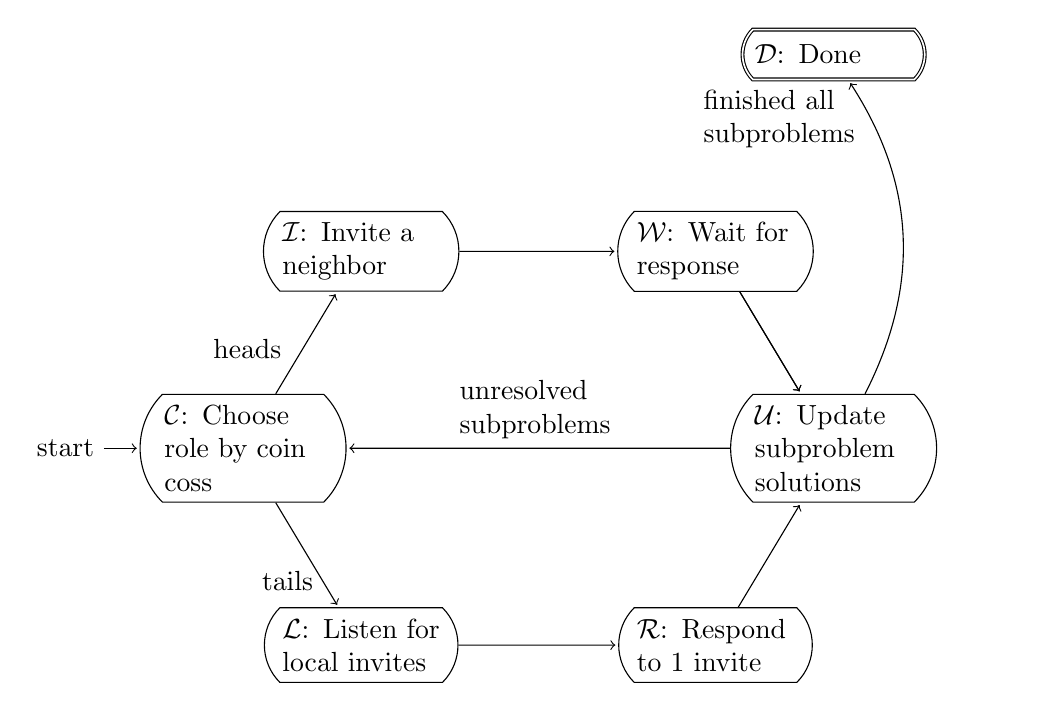
\begin{tikzpicture}[shorten >=1pt,node distance=1cm,on grid,auto, bend angle=75, every state/.style={scale=1, minimum size=18pt, inner sep=2pt}]
    %\draw [help lines] (-5,-4) grid (7,4);
    \path [help lines] (-4,-4) grid (7,4);
		
    \node [rst, initial]   (C) at (-3,-1) {\cCd: Choose role by coin coss};
    \node [rst] (I)            at (-1.5,1.5) {\cId: Invite a neighbor};
    \node [rst] (L)            at (-1.5,-3.5) {\cLd: Listen for local invites};
    \node [rst] (W)            at (3,1.5)  {\cWd: Wait for response};
    \node [rst] (R)            at (3,-3.5) {\cRd: Respond to 1 invite};
    \node [rst] (U)            at (4.5,-1) {\cUd: Update subproblem solutions};
    \node [rst, accepting] (D) at (4.5,4)  {\cDd: Done};

    \path [->] (C) edge              node [near start] {heads} (I)
               (C) edge              node [near end, left] {tails} (L)
               (L) edge              node {} (R)
               (I) edge              node {} (W)
               (W) edge              node {} (U)
               (R) edge              node {} (U);
    \path [->] (U) edge [bend right=30]             node [very near end, left, text width=2cm] {finished all subproblems} (D);
    \path [->] (W) edge  node {} (U);
    \path [->] (U) edge  node [above, text width=2cm] {unresolved subproblems} (C);

  \end{tikzpicture}
  \caption{Distributed Matching and Computation Automata}
  \label{fig:automata}
  \end{center}
\end{figure}


Each node begins a decision round in the \cCd, or {\em choose} state, and chooses randomly whether to transition to the \cId\ or \cLd\ state. Nodes in the \cId\ state choose a single neighbor with a shared subproblem (such as covering or coloring a shared edge) and issue an {\em invitation} to solve that subproblem in this round. 

An invitation should contain all of the information that the invitee needs to compute the solution to the subproblem for this round. For example, if the problem being solved is edge coloring, a node would send it's own id, the id of the intended receiver, and a set of potential colors. Nodes in the \cLd\ state collect any invitations addressed to them. 

In the next step, each node that was in the \cLd\ state transitions to the \cRd\ state, chooses a single invitation from their collection and responds to that invitation. An invitation response is essentially a mirror of the original invitation, containing the id of the responding node, the id of the original sender, and an acceptable solution to the subproblem. 

Nodes in the \cId\ state transition to \cWd\ state and filter incoming messages for the response to the invitation that they sent in the previous step. 

Finally, all nodes transition to the \cUd\ state, solve their local subproblem, and broadcast their solutions. Nodes with no outstanding problems to be solved transition to \cDd\ and terminate, nodes with outstanding sub-problems go back to \cCd.


\subsection{Prior Work}

\subsubsection{Vertex Cover}

Sequential Linear time algorithms for covering problems are surveyed in detail in \cite{254190}. The seminal paper on Linear Programming techniques for constant ratio approximation of MWVC was published by Bar-Yehuda and Even in 1981 \cite{Bar-Yehuda:1981lr}. Gonzalez created a 2-approximate LP-Free linear time algorithm based on Maximal Matching in 1995 which is the basis of our distributed algorithm \cite{Gonzalez1995129}. 

We are aware of three prior distributed algorithms for minimum weighted vertex cover. Grandoni et. al present a 2-approximate algorithm based on maximal matching in 2008\cite{1435381}. This algorithm uses $O(\log n + \hat{W})$ communication rounds, where $\hat{W}$ is the average vertex weight, and $n$ is the number of vertexes. {\AA}strand and Suomela presented a $O(\Delta + \hat{W})$ deterministic algorithm in 2010 which is also 2-approximate. Koufogiannakis and Young present a simpler $O(\log n)$ algorithm in 2009 \cite{1582746}. 

Parnas and Ron proved in 2007 that the query complexity of a randomized algorithm for solving MWVC in a message passing model grows linearly with the average degree of the graph\cite{Parnas:2007:AMV:1280283.1280327}. Following that work, Onak, Ron, Rosen and Rubinfeld present a deterministic algorithm that is 2-approximate in $O(\delta)$ time, where $\delta$ is the average degree of the graph\cite{Onak:2012:NSA:2095116.2095204}. 


\subsubsection{Edge Coloring}

Distributed edge coloring is a well studied problem. Panconesi and collaborators have produced a number of papers tying edge coloring to channel assignment and presenting novel edge coloring algorithms with communication complexity of as low as $O(log{log{n}})$ \cite{Grable:1997:NOD:314161.314266},\cite{Panconesi:1997:RDE:249364.249368},\cite{1041515},\cite{982945}.

Gandham et al. present an deterministic algorithm which colors a graph using $\Delta + 1$ colors with a time complexity of $2\Delta + 1$ for acyclic graphs \cite{1498534}. Barenboim et al. present a deterministic algorithm which extends beyond trees and provides an $O(\Delta)$ coloring in $O(\Delta^{1 + \epsilon})$ time for an arbitrarily small constant $\epsilon \le 1$ \cite{Barenboim:2011:DDE:1993806.1993825}. A limitation of this algorithm is that the constant factor for quality increases as $\epsilon$ decreases.

In strong edge coloring, Barret et al. present algorithms with running times dependent on the size of the graph $n$ \cite{1598948}. Kanj et al. show tight bounds for the quality and locality, but not the time bounds, of their algorithms \cite{Kanj:2009:LAE:1696884.1696902}.


\section{The Vertex Cover Problem}

In this section we'll present the findings for Vertex Cover.

\subsection{Algorithm}
\label{sec:dgmm-description}

Algorithm~\ref{alg:dgmm} is our distributed implementation of the 2-optimal minimum weighted vertex cover algorithm presented by Gonzalez \cite{Gonzalez1995129}. The Gonzalez algorithm, Generalized Maximal Matching for MWVC (or GMM), proceeds by selecting each edge in turn and choosing one of the endpoints of that edge to add to the cover. The sequential algorithm goes through each edge in turn and assigns the edge a weight according to~\eqref{eqn:gmm}.

\begin{align}
  \label{eqn:gmm}
  w(e(u,v)) = min 
  \begin{dcases} 
    w(u) - \sum_{i \ne v} w(e(u,i)) \\
    w(v) - \sum_{i \ne u} w(e(i,v)) 
  \end{dcases} \nonumber \\ 
\intertext{where } 
   w(e(u,i))\text{ or } w(e(i,v)) = 0 \nonumber
\intertext{for unweighted edges}
\end{align}


So if there are no previously weighted edges incident to either endpoint, the weight of the edge is $min(w(u),w(v))$. A vertex $u$ joins the cover when, for all it's weighted edges: \begin{equation}\sum_i w(e(u,i)) = w(u) \label{eqn:sat} \end{equation} When~\eqref{eqn:gmm} is applied to subsequent unweighted incident edges of $u$, the result will be 0. The algorithm terminates when each edge has been weighted. 

In GMM, every edge is examined exactly once. If no endpoints of the edge are in the cover, one endpoint will join the cover. Finally, all the edges are evaluated in arbitrary order. We explore this third point further in Section~\ref{ssb:algorithms-dgmm-performance}. 

Our distributed version of the algorithm chooses some disjoint set of edges (a matching) and assigns weights to those edges according to~\eqref{eqn:gmm}. The framework automata is used to construct the set of disjoint edges in the following manner.\footnote{For the following description, we will substitute the symbol $\varpi(u)$ for the term $\sum_i w(e(u,i))$ in~\eqref{eqn:gmm}.\label{fn:varpi}}

Each node begins in the \cCd\ state. In the first step, each node chooses to transition to state \cId\ or \cLd\ with equal probability. Each node $u$ in the \cId\ state chooses an unweighted edge $e(u,v)$ at random, and broadcasts an invitation containing its incident edge weight ($\varpi(u)$)\footnotemark[\value{footnote}] and the edge it wants to weight. Each node $v$ in the \cLd\ state collects the invitations that contain an edge $e(i,v)$.

For the next step, nodes in the \cLd\ state transition to the \cRd\ state, and nodes in the \cId\ state transition to the \cWd\ state. Each node $v$ in the \cLd\ state chooses an invitation it collected in the prior step and issues a response containing $\varpi(v)$ and the edge $e(u,v)$ that it agrees to weight. Each node in the \cWd\ state filters these responses for the one containing an edge $e(u,i)$ (that is, a response to the invitation it sent in the prior round). 

At this point, there are a number of node pairs in the graph, every node $u$ that sent an invitation to weight an edge $e(u,v)$ forms a pair with $v$ if $v$ responds with an agreement to weight $e(u,v)$. The edges that will be weighted in this round are a matching.

Every node now transitions to the \cUd\ state. Those that have formed node pairs weight the edge $e(u,v)$ according to~\eqref{eqn:gmm}. One of $u,v$ will join the cover at this point. For brevity, in Algorithm~\ref{alg:dgmm}, the \cUd\ state is implied in lines~\algref{alg:dgmm}{alglin:dgmm-update-weight-R} and \algref{alg:dgmm}{alglin:dgmm-update-weight-W}.

Every node now transitions to the \cEd\ state, and broadcasts its current status to its neighbors. If a node $v$ receives a message that a neighbor $u$ has joined the cover $v$ will assign a weight of 0 to $e(u,v)$ and remove $e(u,v)$ from its list of unweighted edges. Again for brevity, the \cEd\ state is executed by implication in lines~\algref{alg:dgmm}{alglin:dgmm-state-E-W} and \algref{alg:dgmm}{alglin:dgmm-state-E}.

Every node that is in the cover now transitions to the \cDd\ state, as does any node that has no unweighted edges remaining. Nodes that still have unweighted edges go back to the \cCd\ state and repeat the process. 


\begin{algorithm}
\caption{Distributed Maximal-Matching-based Minimum-Weighted Vertex Cover  Algorithm (DGMM)}
\begin{algorithmic}[1]
%\Require {$G(V,E)$: a Communication Network}
\ForAll {$v_u \in V$ in parrallel}
\State $S_u \leftarrow False$ \Comment $u$ is not in the cover
\State state $\leftarrow$ \cCd
\Repeat
\State Broadcast $S_u$
\If {$S_v = True$ for $v_v$ incident to self}
\State Set Weight $e_{u,v} \leftarrow 0$ \label{alglin:dgmm-state-E}
\EndIf
\If {state = \cCd}
\State {State $\gets (\cI \lor \cL)$} \Comment Coin toss selects state
\ElsIf {state = \cId}
\State {Randomly select an unweighted edge, $e_{u,v}$}\label{alglin:dgmm-issue-invite}
\State {Broadcast $I_u^v\varpi(u)$} \Comment $u$ Invites $v$ to weight $e_{u,v}$ \label{alglin:dgmm-invite}
\State {state $\leftarrow$ \cWd}
\ElsIf {state = \cLd}
\State {Recieve $I_x^y$} \Comment all local invites
\If {$y = u$} \Comment invite is targeted to $v_u$
\State {store $I_x^y$}
\EndIf
\State {State $\gets \cR$}

\ElsIf {state = \cRd}
\State {Randomly Select $I_v^u$} \Comment from stored invites \label{alglin:dgmm-choose-invite}
\State {Broadcast $R_u^v$} \Comment $u$ accepts $v's$ invitation
\State {Update Weight $e_{u,v}$} \Comment by Equation~\ref{eqn:gmm} \label{alglin:dgmm-update-weight-R}

\If {$\sum w(e(i,u)) = w(u)$}\label{alglin:dgmm-join-cover-R}
\State {$S_u \gets true$} \Comment $u$ joins the cover
\State {Set all unweighted edges to 0} 
\State {state $\gets \cD$}
\Else 
\State {state $\gets \cC$}
\EndIf

\ElsIf {state = \cWd}
\State {Recieve $R_x^y$} \Comment all local responses

\If {$y = u$} \Comment response is to $v_u$
\State {Update Weight $e_{u,v}$}\label{alglin:dgmm-update-weight-W}

\If {$\sum w(e(i,u)) = w(u)$}\label{alglin:dgmm-join-cover-W}
\State $S_u \leftarrow true$ \Comment $u$ joins the cover
\State {Set all unweighted edges to 0}\label{alglin:dgmm-state-E-W}
\State {state $\leftarrow$ \cDd}
\Else 
\State {state $\leftarrow$ \cCd}
\EndIf

\EndIf

\EndIf

\Until {$S_u = true$ OR $S_v = true$  $\forall v_v$ incident $v_u$}\label{alglin:dgmm-end-while}
\EndFor
\end{algorithmic}
\label{alg:dgmm}
\end{algorithm}

\subsection{Analysis}

\label{ssb:algorithms-dgmm-performance}

Despite its overall simplicity, Algorithm~\ref{alg:dgmm} has a running time of $O(\log \Delta)$, which improves on the previous best result of $O(\log n)$ in \cite{1582746} without sacrificing the performance bound of two-optimality. A formal proof of our performance claims follows.

\begin{thm}
  Algorithm~\ref{alg:dgmm} (DGMM) will generate a 2-optimal cover in $O(log \Delta)$ communication rounds with high probability on random input.
\label{thm:dgmm-term}
\end{thm}

\begin{proof}[Proof of Theorem~\ref{thm:dgmm-term}]
\label{prf:correct}

\begin{lem}
\label{lem:dgmm-edge}
  DGMM weights each edge once in a manner equivalent to GMM.
\end{lem}


\begin{lem}
\label{lem:dgmm-log}
Algorithm~\ref{alg:dgmm} (DMMW) terminates in $O(log \Delta)$ rounds with high probability for random connected graphs.
\end{lem}


\begin{proof}[Proof of Lemma~\ref{lem:dgmm-log}]
\begin{ldef}
A node is {\em committed} if it has joined the cover or if all of its neighbors have joined the cover.
\end{ldef}
\begin{ldef}
A node is {\em active} if it is not committed.
\end{ldef}
\begin{ldef}
$\Delta$ is the maximum degree of the Graph.
\end{ldef}

\begin{ldef}
The active degree of a node $u$ is the number of unweighted edges of $u$ indicated by $\alpha(u)$. $\alpha(u)$ is either 0 for committed nodes or equal to the number of active neighbors of $u$ for active nodes.
\end{ldef}
\begin{ldef}
$\delta$ is the largest active degree in the graph.
\end{ldef}

Lemma~\ref{lem:dgmm-log} can be restated in terms of the following propositions:
\begin{lprp}
\label{prop:dgmm-log-each}
Each active node in the graph joins the cover with a constant probability in each round.
\end{lprp}
\begin{lprp}
\label{prop:dgmm-log-alpha}
With high probability, $\delta$ decreases by a constant fraction in each round.
\end{lprp}
\begin{proof}[Proof of Proposition~\ref{prop:dgmm-log-each}]

We begin with a node, $w$, which is an active node in the graph. We want to show that the probability that $w$ will join the cover is constant. Let us assume that $w$ chooses to be a receiver, an event which happens with $P(0.5)$

We know that $w$ has some number of active neighbors, indicated by $\alpha(w)$. Each neighbor of $w$ also has some number of active neighbors. Each active degree is an integer between 1 and $\delta$. We can consider each node to have approximately the same active degree, which we indicate by $\alpha$. 

Each active neighbor of $w$ also chooses to be a sender or a receiver with equal probability. Following the assumption of equal distribution, there are $\sfrac{\alpha}{2}$ senders in the neighborhood of $w$, and each sender has $\alpha$ neighbors.

Each neighbor of $w$ that chooses to be a sender will, according to Line~\ref{alglin:dgmm-issue-invite} of Algorithm~\ref{alg:dgmm}, choose one neighbor which is active and send an invitation to that node. Because there are approximately $\sfrac{\alpha}{2}$ inviting neighbors of $w$, we can consider the probability that $w$ will recieve an invitation to be approximately equivalent to the probability that any event with a probability of $\sfrac{1}{n}$ will occur in $\sfrac{n}{2}$ independent trials for $n > 0$. 

Therefore, the probability that $w$ will recieve an invitation from an active neighbor is: \begin{equation}
1 - \left(\frac{n-1}{n}\right)^{\frac{n}{2}} > \lim_{0 \to \infty} 1 - \left(\frac{k-1}{k}\right)^{\frac{k}{2}} = 1 - \frac{1}{\sqrt{{\mathrm{e}}}} \approx 0.393
\end{equation}


If $w$ recieves at least one invitation, it will respond to exactly one invitation (\algref{alg:dgmm}{alglin:dgmm-choose-invite}), so the probability that $w$ will respond to an invitation from some active neighbor $v$ is exactly the same as the probability that $w$ will recieve an invitation from some active neighbor $v$. Therefore, if $w$ is a receiver, $w$ joins the cover with a probability of $1 - \sfrac{1}{\sqrt{{\mathrm{e}}}}$, which is constant. The probability of $w$ being a receiver at all is $\sfrac{1}{2}$, and the probability of $w$ joining the cover is also $\sfrac{1}{2}$, as we assume that weights are distributed arbitrarily through the graph. Therefore, the probability that $w$ will join the cover in any given round is constant.
\end{proof}

\begin{proof}[Proof of Proposition~\ref{prop:dgmm-log-alpha}]

We consider a node $u$, where $\alpha(u) = \delta$. $u$ may choose to be a sender or a receiver in this round, and $u$ may or may not join the matching. We do make the assumption that $u$ does not join the cover in this round.

$u$ has $\delta$ active neighbors. According to Proposition~\ref{prop:dgmm-log-each}, each of these neighbors joins the cover with constant probability. So in round one, we expect some constant percentage $p$ of the neighbors of $u$ to join the cover, and some constant percentage $q = 1-p$ of the neighbors of $u$ to remain active. Therefore, the value of $\delta(n+1)$ (where $n+1$ represents a round number) is $\delta(n) \times q$. Therefore $\alpha$ decreases at a constant rate, which is what we wanted to show.

\end{proof}

\begin{cor}WHP, the number of communication rounds required to resolve Algorithm~\ref{alg:dgmm} for a random graph is $O(\log\Delta)$.\end{cor}

\end{proof} 

Therefore, because DGMM weights all edges and assigns nodes to the cover in a manner equivalent to GMM in $O(log \Delta)$ communication rounds for random graphs, Theorem~\ref{thm:dgmm-term} is proved.
\end{proof}


\subsection{Experimental Design and Results}

In order to test our performance predictions, we designed a simulator to implement our algorithm (DGMM) and the algorithm of Koufoganiakkis and Young (K/Y). We generated random weighted graphs for $n=120, n=240, n=480, \text{and } n=960$, with average degrees of 3, 6, 12, 24, 48 and 96. 50 graphs were generated for each combination of sizes and average degree, for a total of 1200 graphs. DGMM and K/Y were used to produce a vertex cover for each graph, and the total weight and number of communication rounds were tallied and averaged for each of the 24 graph sizes. Our results showed that DGMM produced covers of approximately the same weight as K/Y in significantly fewer communication rounds in each case. Figures~\ref{plt:dgmm-comp} and \ref{plt:mwvc-rn} show our experimental results.

\begin{figure}[htp]
\begin{center}
\begin{tikzpicture}
  \begin{axis}[xlabel=Average Degree, ylabel=Communication Rounds, legend style={at={(0.95,0.95)}, font=\footnotesize, label={[font=\footnotesize]left:K/Y}, anchor=north east}, legend columns=2, cycle list name={four-1-0}]
    \addplot+[grt] table [x=links, y=star-reg]{\runsone};
    \addplot+[grt] table [x=links, y=star-reg]{\runstwo};
    \addplot+[grt] table [x=links, y=star-reg]{\runsthree};
    \addplot+[grt] table [x=links, y=star-reg]{\runsfour};
    \addplot+[inv] table [x=links, y=mat-reg]{\runsone};
    \addplot+[inv] table [x=links, y=mat-reg]{\runstwo};
    \addplot+[inv] table [x=links, y=mat-reg]{\runsthree};
    \addplot+[inv] table [x=links, y=mat-reg]{\runsfour};
    \legend{(120),(240),(480),(960)}
  \end{axis}
  \begin{axis}[axis x line=none, axis y line=none, legend style={at={(0.05,0.425)}, font=\footnotesize, label={[font=\footnotesize]above left:DGMM}, anchor=north west}, legend columns=2, cycle list name={four-0-1}]
    \addplot+[inv] table [x=links, y=star-reg]{\runsone};
    \addplot+[inv] table [x=links, y=star-reg]{\runstwo};
    \addplot+[inv] table [x=links, y=star-reg]{\runsthree};
    \addplot+[inv] table [x=links, y=star-reg]{\runsfour};
    \addplot+[bls] table [x=links, y=mat-reg]{\runsone};
    \addplot+[bls] table [x=links, y=mat-reg]{\runstwo};
    \addplot+[bls] table [x=links, y=mat-reg]{\runsthree};
    \addplot+[bls] table [x=links, y=mat-reg]{\runsfour};
    \legend{,,,,(120),(240),(480),(960)}
  \end{axis}
\end{tikzpicture}

\caption{Rounds to resolve MWVC}
\label{plt:mwvc-rn}
\end{center}
\end{figure}

\begin{figure}[htp]
\begin{center}
\begin{tikzpicture}
  \begin{axis}[xlabel=Average Degree, ylabel=Total Weight, legend style={at={(.95,.69)}, label={[font=\footnotesize]left:K/Y}, font=\footnotesize, anchor=south east}, legend columns=2, cycle list name={four-1-0}]
    \addplot+[grt] table  [x=links, y=star-reg]{\averageone};
    \addplot+[grt] table  [x=links, y=star-reg]{\averagetwo};
    \addplot+[grt] table  [x=links, y=star-reg]{\averagethree};
    \addplot+[grt] table  [x=links, y=star-reg]{\averagefour};
    \addplot+[inv] table [x=links, y=mat-reg]{\averageone};
    \addplot+[inv] table [x=links, y=mat-reg]{\averagetwo};
    \addplot+[inv] table [x=links, y=mat-reg]{\averagethree};
    \addplot+[inv] table [x=links, y=mat-reg]{\averagefour};
    \legend{(120),(240),(480),(960)}
  \end{axis}
  \begin{axis}[axis x line=none,axis y line=none, legend style={at={(.95,.68)}, label={[font=\footnotesize]left:DGMM}, font=\footnotesize, anchor=north east}, legend columns=2, cycle list name={four-0-1}]
    \addplot+[inv] table  [x=links, y=star-reg]{\averageone};
    \addplot+[inv] table  [x=links, y=star-reg]{\averagetwo};
    \addplot+[inv] table  [x=links, y=star-reg]{\averagethree};
    \addplot+[inv] table  [x=links, y=star-reg]{\averagefour};
    \addplot+[bls] table [x=links, y=mat-reg]{\averageone};
    \addplot+[bls] table [x=links, y=mat-reg]{\averagetwo};
    \addplot+[bls] table [x=links, y=mat-reg]{\averagethree};
    \addplot+[bls] table [x=links, y=mat-reg]{\averagefour};
    \legend{,,,,(120),(240),(480),(960)}
  \end{axis}
\end{tikzpicture}


\caption{Average Weights For MWVC}
\label{plt:dgmm-comp}
\end{center}
\end{figure}


In Figure~\ref{plt:dgmm-comp}, the results for both algorithms are nearly identical, indicating that both algorithms found essentially the same covers for the input graphs. In Figure~\ref{plt:mwvc-rn}, the lower 4 curves indicate the number of rounds required to resolve DGMM, and the upper four the number of rounds required to resolve K/Y. The logarithmic growth confirms our experimental predictions, while the minor differences between different input sizes are accounted for by the variation in degree between larger and smaller random graphs.


\section{Edge Coloring Problem}

In this section we'll present the approach for edge coloring.

\subsection{Distance 1 Algorithm}
\subsubsection{Description}
\begin{algorithm}
\caption{Distributed Matching Based Edge-Coloring Algorithm}
\begin{algorithmic}[1]
%\Require {$G(V,E)$: a Communication Network}
\ForAll {$v_u \in V$ in parrallel}
\State {$live_u \gets C$} \Comment All colors are available \label{alglin:ec-init-color}
\State {$dead_u \gets \{\}$} \Comment No colors are used \label{alglin:ec-init-dict}
\State {$used_u \gets [\,]$} \Comment No colors are assigned
\State state $\leftarrow$ \cCd
\Repeat
\If {state = \cCd}
\State {State $\gets (\cI \lor \cL)$} \Comment Coin toss selects state

\ElsIf {state = \cId}
\State {Randomly select an uncolored edge, $e_{u,v}$}\label{alglin:ec-issue-invite}
\State {$c \gets (live_u \smallsetminus used_v[1]$} \Comment assign first available color to $c$ \label{alglin:ec-select-color}
\State {Broadcast $I_u^v,c$} \Comment $u$ Invites $v$ to color $e_{u,v} \text{ with } c$ 
\State {state $\leftarrow$ \cWd}

\ElsIf {state = \cLd}
\State {Recieve $I_x^y,c$} \Comment all local invites
\If {$y = u$} \Comment invite is targeted to $v_u$
\State {store $I_x^y,c$}
\EndIf
\State {State $\gets \cR$}

\ElsIf {state = \cRd}
\State {Randomly Select $I_v^u,c$} \Comment from stored invites \label{alglin:ec-choose-invite}
\State {Broadcast $R_u^v,c $} \Comment $u$ accepts $v's$ invitation
\State {Assign $c \mapsto e_{u,v}$} 
\State {$used_u \hookleftarrow c$} \Comment Append c to assigned colors \label{alglin:ec-assign1}
\State {state $\gets \cU$}

\ElsIf {state = \cWd}\label{alglin:ec-receive-responses}
\State {Recieve $R_x^y,c$} \Comment all local responses
\If {$y = u$} \Comment response is to $v_u$ 
\State {Assign $c \mapsto e_{u,v}$} 
\State {$used \hookleftarrow c$} 
\EndIf
\State {state $\gets \cU$}

\ElsIf {state = \cUd}
\State {Broadcast $used_u$} \Comment Broadcast all assigned edge colors
\State {Recieve $used_v$} \Comment Receive neighbors assigned colors
\State {$dead_u \hookleftarrow used_v$}  \Comment the "dead" set contains the used colors from each neighbor, and is used when choosing colors in the invitation step \label{alglin:ec-assign2}
\State {state $\gets \cE$}

\ElsIf {State = \cEd}
\State {Subtract $used_u$ from $live_u$} \Comment update usable colors \label{alglin:ec-update-colors}
\State {state $\gets \cC$}

\EndIf
\Until {All edges are assigned a color}\label{alglin:ec-end-while}
\EndFor
\end{algorithmic}
\label{alg:edge-color}
\end{algorithm}


\label{sec:dimaed-description}
In Figure~\ref{fig:automata}, the states of the vertexes are labeled \cCd, \cId, \cLd, \cWd, \cRd, \cUd, and \cDd. In our adaptation of the automata, shown in Algorithm~\ref{alg:edge-color}, an additional state, \cEd, is used for the purposes of exchanging information at the end of each round.

Each node maintains a list of colors that each of its neighbors has used. This is updated at the end of each round.

All transitions are made synchronously, that is, we assume that if any node in the network is in a given state, all nodes in the network are either in that state or in a corresponding state. States that correspond are \{\cCd, \cDd\}, \{\cId, \cLd\}, \{\cRd, \cWd\}.

\paragraph{\cCd\ (Choose) state}
Each vertex chooses with equal probability to transition to the \cId\ state or the \cLd\ state. 

\paragraph{\cId\ (Invite) State} 
Each node in the \cId\ state chooses an available edge and available color. The edge is chosen randomly from among the nodes uncolored edges, and the color is the lowest indexed color available to color that edge (Algorithm~\ref{alg:edge-color}, lines~\algref{alg:edge-color}{alglin:ec-select-color},\algref{alg:edge-color}{alglin:ec-assign2}). The node then sends a message containing its own id, the id of the intended receiver, and the proposed color. 

\paragraph{\cLd\ (Listen) State} 
Each Node in the \cLd\ state listens for invitations from its neighbors. From among the invitations received, the node will keep invitations containing its own id and transition to the \cRd\ state.

\paragraph{\cRd\ (Respond) State}
Each node in the \cRd\ state chooses a random invitation from the invitations received and kept in the \cLd\ state. The node sends a reply message containing its own id, the id of the original sender, and the proposed color from the invitation. This response message is a duplicate of the invitation message with the ids reversed. The node then transitions to the \cUd\ state. Nodes that received no invitations simply transition to the \cUd\ state.

\paragraph{\cWd\ (Wait) State}
Nodes in the \cWd\ state collect all replies in their neighborhood and transition to the \cUd\ state.

\paragraph{\cUd\ (Update) State}
Nodes in the \cUd\ state update their own edges if they have received a response to an invitation or responded to an invitation. All nodes next transition to the \cEd\ state. 

\paragraph{\cEd\ (Exchange) State}
In this state, nodes that have used new colors broadcast those colors to their neighbors. All nodes use this information to update the colors that they have available to exchange with their neighbors. Nodes which have colored all of their edges transfer to the \cDd\ (Done) State, and all other nodes transition back to \cCd.


\subsubsection{Analysis}
We here address the termination, correctness, and solution quality of Algorithm~\ref{alg:edge-color}. We will first show that Algorithm~\ref{alg:edge-color} is likely to terminate in $O(\Delta)$ rounds, then that it will produce a correct coloring if it does terminate, and finally that the coloring produced will use no more than $2\Delta - 1$ colors.
\begin{proof}
We first show that Algorith~\ref{alg:edge-color} terminates in $O(\Delta)$ rounds.

\begin{lem}
\label{lem:edge-color-terminate}
Algorithm~\ref{alg:edge-color} is likely to terminate in $O(\Delta)$ rounds.
\end{lem}

\begin{proof}[Proof of Lemma~\ref{lem:edge-color-terminate}]

Algorithm~\ref{alg:edge-color} terminates when all of the nodes have colored all of their edges. In order to color an edge, a node must form a pair in an a given round with each of its neighbors. The number of neighbors of each node is $\delta \le \Delta$.

We note that there is no limit on the number of nodes that can participate in any given round. If a particular graph has a complete matching, than every compute node may participate in a round. Further, the fact that a node is participating guarantees that at least one of its neighbors is participating, but does not prevent any of its other neighbors from participating as well.

Therefore, if the probability that a given node $w$ will participate in the computation for a given round can be shown to be constant, than the number of compute rounds is bounded by that constant times $\Delta$.

We therefore will procede to find the probability that a random node $w$ will color one of its edges in some round $r$.

Following the same reasoning as the proof of Lemma~\ref{lem:dgmm-log}, we know that in any given round, a which is a receiver will receive an invitation with a constant probability, as shown in Equation~\ref{eqn:bootstrap}. Nodes choose to be a receiver with constant probability, and any node which is a receiver and receives at least one invitation will respond to one invitation.

Therefore the probability that a node will be in the matching in a given round is constant.

A node in the matching will color at least one edge, and no node has more than $\Delta$ edges, so Algorithm~\ref{alg:edge-color} will terminate in $O(\Delta)$ rounds.

\end{proof}

We will now show that the coloring produced by Algorithm~\ref{alg:edge-color} is guaranteed to be correct.
\begin{lem}
\label{lem:edge-color-correct}
Algorithm~\ref{alg:edge-color} produces a correct coloring. 
\end{lem}
\begin{proof}[Proof of Lemma~\ref{lem:edge-color-correct}]

Assume that Algorithm~\ref{alg:edge-color} does not produce a correct coloring, There are two cases where this could occur: either there exists a node $v$ that uses some color twice, or there exist nodes $v,w$ that color the edge $(v,w)$ with different colors. 

A vertex colors an edge after negotiation with some neighbor. In order for an edge to be colored, a vertex $v$ must send an invitation to some neighbor $w$ to color $(v,w)$ with a specific color. Because we assume a message passing model, we assume that $w$ recieves this invitation. If $w$ responds to the invitation, $v$ assigns the color and $w$ assigns the color. In the message passing model, it is safe to assume that $v$ recieves the response from $w$. In order for $v$ to choose a different color than $w$ for $(v,w)$, $v$ would have to either color the edge without a response, which is contrary to the behavior of the vertex (line~\algref{alg:edge-color}{alglin:ec-receive-responses}), or $v$ must not receive the message, which is contrary to our model.

In the second case, a vertex could use the same color twice if it either issued or responded to an invitation to use a color twice. We know, however, that whenever an algorithm uses a color, that color is assigned to a list (lines~\algref{alg:edge-color}{alglin:ec-assign1},~\algref{alg:edge-color}{alglin:ec-assign2}). These colors are further removed from the list in each round (line~\algref{alg:edge-color}{alglin:ec-update-colors}).

If a vertex responded to or issued more than one invitation in a single round, it is possible that this conflict could occur, but this also contradicts the behavior of the algorithm of building a message containing a single id in either case.

Algorithm~\ref{alg:edge-color} therefore produces a correct coloring.
\end{proof}

We now show that the coloring produced by Algorithm~\ref{alg:edge-color} can be no worse than $2\Delta - 1$ in the worst case.
\begin{lem}
\label{lem:edge-color-approximate}
Algorithm~\ref{alg:edge-color} will use $2\Delta - 1$ colors in the worst case. 
\end{lem}

\begin{proof}[Discussion of Lemma~\ref{lem:edge-color-approximate}]

We begin by showing the worst case performance of Algorithm~\ref{alg:edge-color}. 

In each round that a node joins a pair, both nodes use the lowest common indexed color to color the edge between them. So in the first round, color 1 will be used for every edge in the matching, in the second round, color 1 or color 2, in the third 1,2, or 3, and so forth. 

So to model our worst possible case, we propose a node $w$ with the following characteristics. First, node $w$ has a degree of $\Delta$ and all of the neighbors of $w$ have a degree of $\Delta$. Second, $w$ does not participate in the matching in the first $\Delta-1$ rounds, but every neighbor of $w$ does. In this way we insure that $w$ cannot form an edge with any neighbor with an index of less than $\Delta-1$. 

In this case, $w$ will be forced to use an additional $\Delta$ colors to connect to each neighbor, and the total number of colors used will be $2\Delta-1$.
\end{proof}

Therefore, Theorem~\ref{thm:edge-color} is correct.
\end{proof}

\begin{con}
\label{lem:edge-color-optimal}
Algorithm~\ref{alg:edge-color} uses $C \le \Delta + 1$ colors in the typical run. 
\end{con}

\begin{proof}[Discussion of Conjecture~\ref{lem:edge-color-optimal}]

A graph can certainly be colored with either $\Delta$ or $\Delta + 1$ colors. If a node $v$ were to be forced to use $\Delta + 2$ colors to color a graph, that would mean that there are two colors of index $\le \Delta$ which are being used by each neighbor of $v$ but not by $v$ itself.

In order for this to happen, there would need to be some round, or sequentially set of rounds, in which all of $v$'s neighbors formed a matching, and $v$ did not. We know from Proposition~\ref{lem:edge-color-terminate} that the odds of a node forming a match in a given round are greater than $\sfrac{1}{4}$, because the odds of a node being an invitor and recieving an invitation are approximately $\sfrac{1}{4}$. We can also easily calculate that the odds of a node being an invitor and sending a successful invitation are no greater than $\sfrac{1}{4}$, since there is a $\sfrac{1}{2}$ chance that a node $w$ will choose to send invitations and a $\sfrac{1}{2}$ chance that the neighbor $w$ sends an invitation to is an invitee.  

So the odds of a node forming a pair at all in a given round are $\sfrac{1}{x}$, $4 \ge x \ge 2$. 

For a given node to not form a pair while all of its neighbors do form pairs is therefore akin to the odds that in a fair coin toss, we first flip heads and then flip tails some arbitrary number of times in a row, or that in a simultaneous coin toss of some number of coins, one is heads while the rest are tails. 

We therefore expect our algorithm to behave well in the following sense: we should get conistent results with similar graphs, the algorithm should color with $\Delta$ or $\Delta + 1$ colors most of the time, and in no experimental case should we ever see the maximum $2\Delta - 1$ colors used.

\end{proof}



\subsubsection{Experimental Results}

In our experimental results, we found that graph structure was a crucial component in determining the quality of solution that we found in any of our algorithms.

\subsubsection{Algorithm~\ref{alg:edge-color} on Erd\"{o}s-R\'{e}nyi Graphs}
Erd\"{o}s-R\'{e}nyi graphs were generated using the iGraph ruby bindings \cite{Gutteridge:2007fk}. Graphs were generated with 200 or 400 nodes, and an average degree of either 4, 8, or 16. 50 graphs were generated for each size.

Consistent with Conjecture~\ref{lem:edge-color-optimal}, $\Delta + 2$ colors were used in only 2 of the 300 runs, and in no run was the number of colors in excess of $\Delta+2$. In the typical run, our algorithm found a coloring with either $\Delta$ or $\Delta + 1$ colors. 

In keeping with our hypothesis, the number of rounds required to terminate the algorithm increased linearly with $\Delta$, and was not affected by the number of nodes in the network. Figure~\ref{plt:erdren-edge} shows this relationship.

\begin{figure}[htp]
\begin{center}
\begin{tikzpicture}
  \begin{axis}[xlabel=Average $\Delta$, ylabel=Rounds, legend style={at={(1,0.25)}, anchor=east}]
    \addplot table [x=delta, y=rounds]{\erdrenone};
    \addplot table [x=delta, y=rounds]{\erdrentwo};
    \legend{200 Nodes, 400 Nodes};
  \end{axis}
\end{tikzpicture}
\caption{Edge Coloring of Erd\"{o}s-R\'{e}nyi Graph}
\label{plt:erdren-edge}
\end{center}
\end{figure}




\subsubsection{Algorithm~\ref{alg:edge-color} on Small World Graphs}
300 small world graphs were generated, 100 each with 16, 64, and 256 nodes, 50 sparse and 50 dense graphs per set. Algorithm~\ref{alg:edge-color} was used to generate an edge coloring for each graph.

Consistent with Theorem~\ref{thm:edge-color}, the number of rounds required to find a coloring increased linearly with $\Delta$ and was not affected by the number of nodes in the graph. Further, the number of colors required to color the graph was less than $2\Delta -1$ in all cases. Figure~\ref{plt:small-world-ec} shows the relationship between $\Delta$, the number of rounds, and the number of nodes.

\begin{figure}[htp]
\begin{center}
\begin{tikzpicture}
  \begin{axis}[xlabel=Average $\Delta$, ylabel=Rounds, legend style={at={(1,0.25)}, anchor=east}]
    \addplot table [x=delta, y=rounds]{\smlwldone};
    \addplot table [x=delta, y=rounds]{\smlwldtwo};
    \addplot table [x=delta, y=rounds]{\smlwldthree};
    \legend{16 Nodes, 64 Nodes, 256 Nodes};
  \end{axis}
\end{tikzpicture}
\caption{Edge Coloring of Small World Graphs}
\label{plt:small-world-ec}
\end{center}
\end{figure}



Conjecture~\ref{lem:edge-color-optimal} was not supported for this set of graphs. In particular, dense graphs with more nodes tended to use more than $\Delta + 1$ colors in most runs. The most colors used in any run was $\Delta + 5$ for a dense graph with 256 nodes. The average $\Delta$ for this group was 44.4. Further analysis of these results is required. 


\subsubsection{Algorithm~\ref{alg:edge-color} on Scale Free Graphs}
\label{sub:experiment:scalefree}
300 scale-free graphs were generated with either 100 or 400 nodes, with alterations in weighting to create increasingly disparate graphs. Algorithm~\ref{alg:edge-color} was used to generate an edge coloring for each graph.

As expected, rounds increased with Delta at what appears to be a constant rate. Interestingly, in contrast to our results on random graphs, on scale-free graphs we did not use more than $\Delta$ colors to color any of the generated graphs.

Figure~\ref{plt:scale-free-ec} shows our results for Experiment~\ref{sub:experiment:scalefree}.

\begin{figure}[htp]
\begin{center}
\begin{tikzpicture}
  \begin{axis}[xlabel=Average $\Delta$, ylabel=Rounds, legend style={at={(1,0.25)}, anchor=east}]
    \addplot table [x=delta, y=rounds]{\sclfreeone};
    \addplot table [x=delta, y=rounds]{\sclfreetwo};
    \legend{100 Nodes, 400 Nodes};
  \end{axis}
\end{tikzpicture}
\caption{Edge Coloring of Scale-Free Graphs}
\label{plt:scale-free-ec}
\end{center}
\end{figure}




\subsection{Distance 2 Algorithm}
\subsubsection{Description}
\label{sub:dima2ed-description}

\label{sec:dima2ed-description}

Algorithm~\ref{alg:ma2ed} (DiMa2Ed) proceeds in a manner similar to Algorithm~\ref{alg:edge-color}, adding the additional \cEd\ step to Fig~\ref{fig:automata} and adding subroutines at different steps. All compute nodes proceed synchronously. We describe the behavior of each node in each state.

\paragraph{\cCd\ (Choose State)}
Each active node (nodes that have not yet assigned colors to each edge) begin each round in the \cCd\ state. In this state, the nodes choose, with equal probability, to transition to the \cId\ or \cLd\ states for the next communication step.

\paragraph{\cId\ (Inviter) State}
If node $v$ is in the \cId\ state it executes Procedure~\ref{alg:ma2ed-crp}, choosing a potential round partner. Round partners are chosen at random from among the uncolored edges $v,u$ of $v$, $v$ chooses a random $u$ and broadcasts $u$ a message containing the id of $v$, the id of $u$, and a proposed color. $v$ then transitions to the \cWd\ state.

\paragraph{\cLd\ (Listen) State}
If a node $v$ is in the \cLd\ state it collects all messages from its neighbors and transitions to the \cRd\ state. 

\paragraph{\cRd\ (Respond) State}
A node $v$ in the \cRd\ State must evaluate all of its invites to look for one that it can respond to. First, invites can be divided into two categories, those which contain the id of $v$ and those which do not. Call the former group group $a$ and the latter group group $b$. $v$ searches group $a$ for a message which proposes a usable color that is not in any proposal from group $b$. $v$ chooses a single message that meets that qualification and rebroadcasts it. $v$ deletes all other messages from memory and transitions to \cUd.

\paragraph{\cWd\ (Wait) State}
In the \cWd\ state, a node checks all messages from its neighbors looking for the message that it sent in the \cId\ state. If it finds such a message, it keeps it, otherwise, it deletes all messages from memory, and transitions to the \cUd\ state.

\paragraph{\cUd\ (Update) State}
Nodes in the update state either retain 1 or 0 messages in memory. If they contain a message in memory, they color the edge described in the message with the color contained in the message, then eliminate that color from their list of usable colors. Nodes then transition to the \cEd\ state.

\paragraph{\cEd\ (Exchange) State}
Every node exchanges the changes to their color lists with their neighbors and updates their own color lists based on what their neighbors have communicated. Nodes which have uncolored edges now transition back to the \cCd state.

\begin{algorithm}
\caption{Distributed Matching Based Distance 2 Edge Coloring for Directed Graphs (DiMa2ED)}
\begin{algorithmic}[1]
%\Require {$G(V,E)$: a Communicaton Network}
\ForAll {$v_u \in V$ in parrallel}
\Repeat
\State {state $ \gets $ nextstate} 
\Case {$state$}
\When {\cCd}
\State {reset variables}
\State {$nextstate \gets \{\cL \lor \cI\}$ } 
\When {\cId}
\State {{\sc ChooseRoundPartner}}
\State{$nextstate \gets \cW$}
\When {\cLd}
\State {Recieve and store messages}
\State {$nextstate \gets \cR$}  
\When {\cRd}
\State {{\sc EvaluateInvites}}
\State {$nextstate \gets \cU_i$} 
\When {\cWd}
\State {Recieve and store messages}
\State{$nextstate \gets \cU_o$} 
\When {$\cU_i, \cU_o$}
\State {{\sc UpdateEdges}}
\State{$nextstate \gets \cE$} 
\When {\cEd}
\State {{\sc UpdateColors}} \label{alg:ma2ed-lin-update}
\State{$nextstate \gets \cC$} 
\EndCase
\State {{\sc Send} $nextmessage$} \label{alg:ma2ed-lin-send}
\Until {$\forall v \text{ incident to } u, e(u,v) \text{ is colored}$}
\EndFor
\end{algorithmic}
\label{alg:ma2ed}
\end{algorithm}

\begin{subalgorithms}
\begin{algorithm}
\caption{ChooseRoundPartner}
\begin{algorithmic}[1]
\State {choose a random uncolored edge $e(u,v)$}
\State {$roundpartner \gets v$}
\State {Choose an open channel $\phi$ for $v$}
\State {$nextmessage \gets$ {$\phi, v, u$}}
\end{algorithmic}
\label{alg:ma2ed-crp}
\end{algorithm}

\begin{algorithm}
\caption{EvaluateInvites}
\begin{algorithmic}[1]
\For  {$m$ in messages collected}
\If {$m$ includes $u$}
\State {$mine[] \gets message$} \Comment Create an array of messages sent to $u$
\Else 
\State {$other[] \gets message$} \Comment Create an array of messages not sent to $u$
\EndIf
\EndFor
\State {$mine[] \gets mine[] \suchthat \phi \notin other$} \Comment Look for color collisions between $mine$ and $other$
\State {Select a message $m$ from $mine$}
\State {$nextmessage \gets {\phi, u, v} \suchthat m\text{ contains } {\phi, v, u}$} \Comment reply to the chosen message
\end{algorithmic}
\label{alg:ma2ed-ei}
\end{algorithm}

\begin{algorithm}
\caption{UpdateEdges}
\begin{algorithmic}[1]
\State {select a message $m \suchthat m \text { contains } roundparter$} \Comment find the reply--if any--to the last invite sent
\If {$m$}
\Case {$state$}
\When {$\cU_i$}
\State {color edge $e(roundpartner, u) \text { with } \phi \text{ from } m$} \Comment color the incoming edge from the round partner
\When {$\cU_o$}
\State {color edge $e(u, roundpartner) \text { with } \phi \text{ from } m$} \Comment color the outgoing edge to the round partner
\EndCase
\EndIf
\State {$nextmessage \gets {edges, u}$}
\end{algorithmic}
\label{alg:ma2ed-ue}
\end{algorithm}

\begin{algorithm}
\caption{UpdateColors}
\begin{algorithmic}[1]
\State {$colorlist \gets colorlist - newcolors$} \Comment update current color list
\For{$m$ in messages collection}
\For{$incolor$, $outcolor$ in $m$}
\State {$newin[].push(in_color)$}
\State {$newout[].push(out_color)$}
\EndFor
\EndFor
\State {$legalin \gets legalin - newin$} \Comment remove neighbors new in colors from legal in colors
\State {$legalout \gets legalout - newout$} \Comment remove neighbors new out colors from legal out colors
\State $nextmessage \gets {v, nil, newout}$
\end{algorithmic}
\label{alg:ma2ed-uc}
\end{algorithm}
\end{subalgorithms}

\subsubsection{Analysis}
We here address the termination and correctness of Algorithm~\ref{alg:ma2ed}.
\begin{thm} Algorithm~\ref{alg:ma2ed} will produce a correct, distance-2 directed coloring in $O(\Delta)$ rounds where $\Delta$ is the maximum degree of the graph.
\label{thm:ma2ed-correct}
\end{thm}

\begin{proof}
\begin{lemm} 
\label{lem:dima2ed-term}
Algorithm~\ref{alg:ma2ed} will terminate in $O(\Delta)$ rounds in the typical case.
\end{lemm}

The proof of Lemma~\ref{lem:edge-color-terminate} applies to Lemma~\ref{lem:dima2ed-term} as well.

\begin{lemm}
\label{lem:ma2ed-color-correct}
Algorithm~\ref{alg:ma2ed} produces a correct coloring.
\end{lemm}
\begin{proof}[Proof of Lemma~\ref{lem:ma2ed-color-correct}]
We proceed by direct contradiction. Suppose that Algorithm~\ref{alg:ma2ed} terminates, but the coloring is not correct. There are two cases where this can happen.
\begin{paragraph}{Case 1} A node uses the same color twice.

Recall that each node colors exactly one outgoing or incoming edge at a time. In order for a single node to use one color for two edges, that node would have to either issue or accept an invite to use a color that it is already using. Since each node checks its legal color list before it issues or accepts an invite, this could only happen if some node used a color but did not update its color list. This contradicts the steps of the algorithm, in particular line~\algref{alg:ma2ed}{alg:ma2ed-lin-update}.
\end{paragraph}
\begin{paragraph}{Case 2} $\exists\ u,v,w,x \in V, (u,v), (v,w), (w,x) \in E \suchthat (u,v) \text{ is using color } \phi \text{ and } (w,x)\text{ is using color } \phi$.

For $(uv)$ and $(wx)$ to be colored simultaneously, node $v$ would have to accept the invitation from node $u$. However, our graph is bidirectional, the existence of $(vw)$ implies the existence of $(wv)$. Therefore, in the round that $v$ accepts the invitation from $u$, it would also collect the invitation from $w$ to $x$. Since $v$ will not accept an invitation if it detects a conflict, $v$ will not accept the invitation from $u$ and the edges cannot be colored simultaneously.

For $(uv)$ and $(wx)$ to be colored in two different rounds, either $v$ must accept the invitation from $u$ after $(wx)$ is colored or $w$ must send an invitation to $x$ after $(uv)$ has been colored. Either case assumes that $v$ or $w$ did not update their legal color lists at the end of some previous round. This contradicts the steps of the algorithm.
\end{paragraph}
If this is true, Lemma~\ref{lem:ma2ed-color-correct} is correct.
\end{proof}



If Lemma~\ref{lem:dima2ed-term} is correct and Lemma~\ref{lem:ma2ed-color-correct} is correct, Theorem~\ref{thm:ma2ed-correct} is true.

\end{proof}


\subsection{Experimental Results}
\label{sub:experiment-erdren-direct}
50 Erd\"{o}s-R\'{e}nyi graphs of 200 and 400 nodes were constructed with an average degree of 4 and 8. The averaged results showed that the graphs with 400 nodes were solved in almost identical time, with any variance easily attributable to a slightly higher average $\Delta$. The degree of increase in the number of rounds required to create a correct distance two coloring was also consistent with the increase in $\Delta$. 

Figure~\ref{plt:erdren-direct-strong} shows the results of experiment~\ref{sub:experiment-erdren-direct}.

\begin{figure}[htp]
\begin{center}
\begin{tikzpicture}
  \begin{axis}[xlabel=Average $\Delta$, ylabel=Rounds, legend style={at={(1,0.25)}, anchor=east}]
    \addplot table [x=delta, y=rounds]{\erddirone};
    \addplot table [x=delta, y=rounds]{\erddirtwo};
    \legend{200 Nodes, 400 Nodes};
  \end{axis}
\end{tikzpicture}
\caption{Strong Edge Coloring of Directed Erdos-Renyi Graph}
\label{plt:erdren-direct-strong}
\end{center}
\end{figure}



\section{Expansion to other problems and problems that cannot be solved in covering/covering}

\bibliographystyle{plain}
\bibliography{ijnc-apdcm-2012}


\end{document}

